\chapter{The Epsilon Merging Language (EML)}
\label{sec:EML}

The aim of EML is to contribute model merging capabilities to Epsilon. More specifically, EML can be used to merge an arbitrary number of input models of potentially diverse metamodels and modelling technologies. This section provides a discussion on the motivation for implementing EML, its abstract and concrete syntax, as well as its execution semantics. It also provides two examples of merging homogeneous and heterogeneous models.

\section{Motivation}

A mechanism that enables automatically merging models on a set of established correspondences has a number of applications in a model driven engineering process. For instance, it can be used to unify two complementary, but potentially overlapping, models that describe different views of the same system. In another scenario, it can be used to merge a core model with an aspect model (potentially conforming to different metamodels), as discussed in \cite{MDAGuide} where a core \emph{Platform Independent Model (PIM)} is merged with a \emph{Platform Definition Model (PDM)}, that contributes platform-specific aspects, into a \emph{Platform Specific Model (PSM)}.

\subsection{Phases of Model Merging}

Existing research \cite{Pottinger2003,Batini1986} has demonstrated that model merging can be decomposed into four distinct phases: comparison, conformance checking, merging and reconciliation (or restructuring).

\paragraph{Comparison Phase} In the comparison phase, correspondences between equivalent elements of the source models are identified, so that such elements are not propagated in duplicate in the merged model.

%In \cite{ModelWeaver} the ModelWeaver, a generic framework for capturing different types of relationships, such as match relationships, between elements of different models is illustrated.  Matching pairs of elements can be defined graphically through a tree-based user interface and declared relationships can be stored in a separate \textit{weaving model}. Weaving models can be used later by other tools such as model transformation or model merging tools. While this is a flexible approach that promotes reuse, it does not scale well since manual definition of each matching pair is a labour intensive process.

%In \cite{Alanen2003}, matching is performed using persistent model-element identifiers (i.e. using the $xmi.id$ identifier). However, this only applies to comparison of models that are versions of a common ancestor. In \cite{Gray2005}, matching is performed by comparing the \textit{names} of the elements of the two models. Nevertheless, there are model elements that do not have a name (e.g. instances of the $Multiplicity$ UML metaclass) to compare.

\paragraph{Conformance Checking Phase} In this phase, elements that have been identified as matching in the previous phase are examined for conformance with each other. The purpose of this phase is to identify potential conflicts that would render merging infeasible. The majority of proposed approaches, such as \cite{Letkeman2005}, address conformance checking of models complying with the same metamodel. 
 
\paragraph{Merging Phase}
Several approaches have been proposed for the merging phase. In \cite{Pottinger2003,Melnik2003}, graph-based algorithms for merging models of the same metamodel are proposed. In \cite{Letkeman2005}, an interactive process for merging of UML 2.0 models is presented. There are at least two weaknesses in the methods proposed so far. First, they only address the issue of merging models of the same metamodel, and some of them address a specific metamodel indeed. Second, they use an inflexible merging algorithm and do not provide means for extending or customizing its logic.

\paragraph{Reconciliation and Restructuring Phase}
After the merging phase, the target model may contain inconsistencies that need fixing. In the final step of the process, such inconsistencies are removed and the model is \textit{polished} to acquire its final form. Although the need for a reconciliation phase is discussed in \cite{Batini1986,Melnik2003}, in the related literature the subject is not explicitly targeted.

\subsection{Relationship between Model Merging and Model Transformation}

A merging operation is a transformation in a general sense, since it transforms some input (source models) into some output (target models). However, as discussed throughout this section, a model merging facility has special requirements (support for comparison, conformance checking and merging pairs of input elements) that are not required for typical \textit{one-to-one} or \textit{one-to-many} transformations \cite{Czarnecki2003} and are therefore not supported by contemporary model transformation languages.

\section{Realizing a Model Merging Process with Epsilon}

The first two steps of the process described above can be realized with existing languages provided by Epsilon. As discussed in Section \ref{sec:ECL}, the comparison step can be realized with the Epsilon Comparison Language (ECL). Following that, the Epsilon Validation Language (EVL) can be used to validate the identified correspondences using the match trace calculated by ECL. The Epsilon Merging Language (EML) presented below provides support for the last two steps of the process (merging and reconciliation/restructuring).

\section{Abstract Syntax}

In EML, merging specifications are organized in modules (\emph{EmlModule}). As displayed in Figure \ref{fig:EmlAbstractSyntax}, \emph{EmlModule} inherits from \emph{EtlModule}.

\begin{sidewaysfigure}
  \centering
  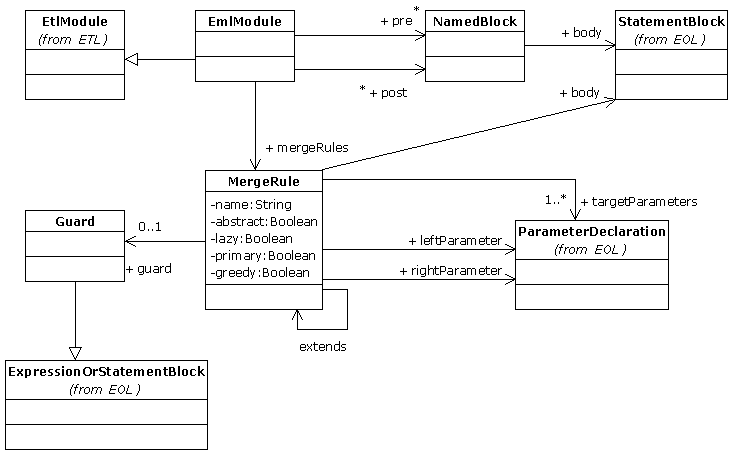
\includegraphics{images/EmlAbstractSyntax.png}
  \caption{The Abstract Syntax of EML}
  \label{fig:EmlAbstractSyntax}
\end{sidewaysfigure}

By extending \emph{EtlModule}, an EML module can contain a number of transformation rules and user-defined operations. An EML module can also contain one or more merge rules as well as a set of \emph{pre} and \emph{post} named EOL statement blocks. As usual, \emph{pre} and \emph{post} blocks will be run before and after all rules, respectively.

Each merge rule defines a name, a left, a right, and one or more target parameters. It can also extend one or more other merge rules and be defined as having one or more of the following properties: abstract, greedy, lazy and primary.

\section{Concrete Syntax}

Listing \ref{lst:EmlConcreteSyntax} demonstrates the concrete syntax of EML merge-rules.

\begin{lstlisting}[caption=Concrete syntax of an EML merge-rule, label=lst:EmlConcreteSyntax, language=EML, escapechar=!]
(@abstract)?
(@lazy)?
(@primary)?
(@greedy)?
rule !\textit{<name>}!
	merge !\textit{<leftParameter>}!
	with !\textit{<rightParameter>}!
	into (!\textit{<targetParameter>}!(!\textbf{,} \textit{<targetParameter>}!)*)?
	(extends !\textit{<ruleName>}!(!\textbf{,} \textit{<ruleName>}!)*)? {

	!\textit{statementBlock}!

}
\end{lstlisting}

\emph{Pre} and \emph{post} blocks have a simple syntax that, as presented in Listing \ref{lst:EmlPrePostConcreteSyntax}, consists of the identifier (\emph{pre} or \emph{post}), an optional name and the set of statements to be executed enclosed in curly braces.

\begin{lstlisting}[caption=Concrete Syntax of Pre and Post blocks, label=lst:EmlPrePostConcreteSyntax, language=EML]
(pre|post) <name> {
	statement+
}
\end{lstlisting}

\section{Execution Semantics}

\subsection{Rule and Block Overriding}
An EML module can import a number of other EML and ETL modules. In this case, the importing EML module inherits all the rules and pre/post blocks specified in the modules it imports (recursively). If the module specifies a rule or a pre/post block with the same name, the local rule/block overrides the imported one respectively.

\subsection{Rule Scheduling}
When an EML module is executed, the \emph{pre} blocks are executed in the order in which they have been defined.

Following that, for each \emph{match} of the established \emph{matchTrace} the applicable non-abstract, non-lazy merge rules are executed. When all \emph{matches} have been merged, the transformation rules of the module are executed on all applicable elements - that have not been merged - in the models.

Finally, after all rules have been applied, the \emph{post} blocks of the module are executed.

\subsection{Rule Applicability}
By default, for a merge-rule to apply to a \emph{match}, the \emph{left} and \emph{right} elements of the match must have a \emph{type-of} relationship with the \emph{leftParameter} and \emph{rightParameter} of the rule respectively. This can be relaxed to a \emph{kind-of} relationship by specifying that the merge rule is \emph{greedy} (using the \emph{@greedy} annotation in terms of concrete syntax).

\subsection{Source Elements Resolution}

As with model transformation, in model merging it is often required to resolve the counterparts of an element of a source model into the target models. In EML, this is achieved by overloading the semantics of the \emph{equivalents()} and \emph{equivalent()} operations defined by ETL. In EML, in addition to inspecting the transformation trace and invoking any applicable transformation rules, the \emph{equivalents()} operation also examines the \emph{mergeTrace} (displayed in Figure \ref{fig:EmlRuntime}) that stores the results of the application of merge-rules and invokes any applicable (both lazy and non-lazy) rules.

Similarly to ETL, the order of the results of the \emph{equivalents()} operation respects the order of the (merge or transform) rules that have produced them. An exception to that occurs if one of the rules has been declared as primary, in which case its results are prepended to the list of elements returned by equivalent.

\begin{figure}
	\centering
		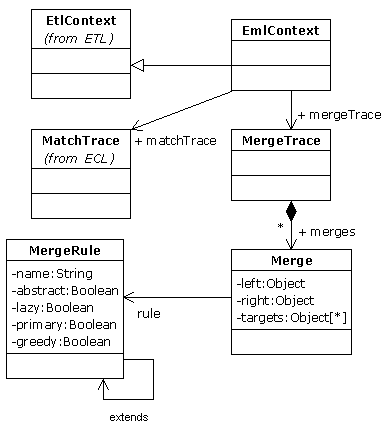
\includegraphics{images/EmlRuntime.png}
	\caption{The EML runtime}
	\label{fig:EmlRuntime}
\end{figure}

\section{Homogeneous Model Merging Example}

In this scenario, two models conforming to the Graph metamodel need to be merged. The first step is to compare the two graphs using the ECL module of Listing \ref{lst:CompareGraph}.

\begin{lstlisting}[caption=ECL module for comparing two instances of the Graph metamodel, label=lst:CompareGraph, language=ECL, tabsize=2]
rule MatchNodes /*@\label{line:MatchNodes}@*/
	match l : Left!Node
	with r : Right!Node {

	compare : l.label = r.label
}

rule MatchEdges /*@\label{line:MatchEdges}@*/
	match l : Left!Edge
	with r : Right!Edge {

	compare : l.source.matches(r.source)
		and l.target.matches(r.target)
}

rule MatchGraphs /*@\label{line:MatchGraphs}@*/
	match l : Left!Graph
	with r : Right!Graph {

	compare : true
}
\end{lstlisting}

The \emph{MatchNodes} rule in line \ref{line:MatchNodes} defines that two nodes match if they have the same label. The \emph{MatchEdges} rule in line \ref{line:MatchEdges} specifies that two edges match if both their source and target nodes match (regardless of whether the labels of the edges match or not as it is assumed that there can not be two distinct edges between the same nodes). Finally, since only one instance of Graph is expected to be in each model, the \emph{MatchGraphs} rule in line \ref{line:MatchGraphs} returns \emph{true} for any pair of Graphs\footnote{Both assumptions can be checked using EVL before matching/merging takes place but this is out of the scope of this example}.

Having established the necessary correspondences between matching elements of the two models, the EML specification of listing \ref{lst:MergeGraphs}.

\begin{lstlisting}[label=lst:MergeGraphs, caption=EML module for merging two instances of the Graph metamodel on the correspondences identified in Listing \ref{lst:CompareGraph} , language=EML]
import "Graphs.etl";

rule MergeGraphs /*@\label{line:MergeGraphs}@*/
	merge l : Left!Graph
	with r : Right!Graph
	into t : Target!Graph {
	
	t.label = l.label + " and " + r.label;
	
}

@abstract
rule MergeGraphElements /*@\label{line:MergeGraphElements}@*/
	merge l : Left!GraphElement
	with r : Right!GraphElement
	into t : Target!GraphElement {
	
	t.graph ::= l.graph;
	
}

rule MergeNodes /*@\label{line:MergeNodes}@*/
	merge l : Left!Node
	with r : Right!Node
	into t : Target!Node 
	extends GraphElements {
	
	t.label = "c_" + l.label;
	
}
rule MergeEdges /*@\label{line:MergeEdges}@*/
	merge l : Left!Edge
	with r : Right!Edge
	into t : Target!Edge 
	extends GraphElements {
	
	t.source ::= l.source;
	t.target ::= l.target;
	
}
\end{lstlisting}

In line \ref{line:MergeGraphs}, the \emph{MergeGraphs} merge rule specifies that two matching Graphs (\emph{l} and \emph{r}) are to be merged into one Graph \emph{t} in the target model that has as a label, the concatenation of the labels of the two input graphs separated using 'and'. The \emph{mergeNodes} rule In line \ref{line:MergeNodes} specifies that two matching Nodes are merged into a single Node in the target model. The label of the merged node is derived by concatenating the c (for common) static string with the label of the source Node from the left model. Similarly, the \emph{MergeEdges} rule specifies that two matching Edges are merged into a single Edge in the target model. The source and target nodes of the merged Edge are set to the equivalents (::=) of the source and target nodes of the edge from the left model.

To reduce duplication, the \emph{MergeNodes} and \emph{MergeEdges} rules extend the abstract \emph{MergeGraphElements} rule specified in line \ref{line:MergeGraphElements} which assigns the \emph{graph} property of the graph element to the equivalent of the left graph.

The rules displayed in Listing \ref{lst:MergeGraphs} address only the matching elements of the two models. To also copy the elements for which no equivalent has been found in the opposite model, the EML module imports the ETL module of Listing \ref{lst:CopyGraph}.

\begin{lstlisting}[caption=The Graphs.etl ETL transformation module, label=lst:CopyGraph, language=ETL]
rule TransformGraph 
	transform s : Source!Graph
	to t : Target!Graph {
	
	t.label = s.label;
	
}

@abstract
rule TransformGraphElement 
	transform s : Source!GraphElement
	to t : Target!GraphElement {
	
	t.graph ::= s.graph;
}

rule TransformNode /*@\label{line:TransformNode}@*/
	transform s : Source!Node
	to t : Target!Node 
	extends TransformGraphElement {
	
	t.label = s.graph.label + "_" + s.label;
}

rule TransformEdge 
	transform s : Source!Edge
	to t : Target!Edge 
	extends TransformGraphElement {
	
	t.source ::= s.source;
	t.target ::= s.target;	
} 
\end{lstlisting}

The rules of the ETL module apply to model elements of both the Left and the Right model as both have been aliased as Source. Of special interest is the TransformNode rule in line \ref{line:TransformNode} that specifies that non-matching nodes in the two input models will be transformed into nodes in the target model the labels of which will be a concatenation of their input graph and the label of their counterparts in the input models.

Executing the ECL and EML modules of Listings \ref{lst:CompareGraph} and \ref{lst:MergeGraphs} on the exemplar models displayed in Figures \ref{fig:LeftGraph} and \ref{fig:RightGraph} creates the target model of Figure \ref{fig:TargetGraph}.

\begin{figure}[h]
	\centering
		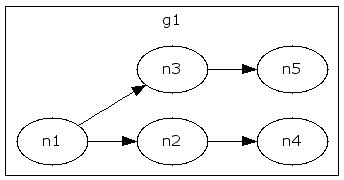
\includegraphics{images/LeftGraph.png}
	\caption{Left input model}
	\label{fig:LeftGraph}
\end{figure}


\begin{figure}[hb]
	\centering
		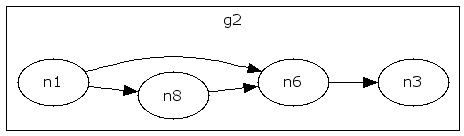
\includegraphics{images/RightGraph.png}
	\caption{Right input model}
	\label{fig:RightGraph}
\end{figure}


\begin{figure}[hb]
	\centering
		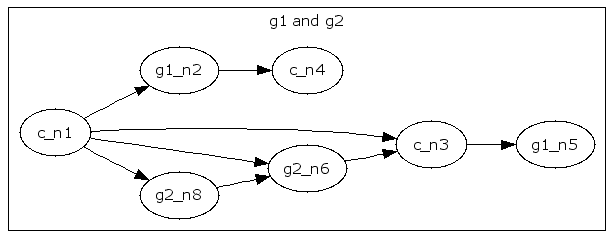
\includegraphics{images/MergedGraph.png}
	\caption{Target model derived by merging the models of Figures \ref{fig:LeftGraph} and \ref{fig:RightGraph}}
	\label{fig:TargetGraph}
\end{figure}